\chapter{Introduction}\label{chap:intro}
\fancyhead[LO]{\nouppercase{\leftmark}}

When considering biomedical time-series data from individuals, understanding and capturing the underlying development patterns on an individual level is the first and essential step towards personalised medicine. Yet, such data are often characterised by a sparse, highly irregular time grid of measurements and individual-specific development patterns, which complicates the corresponding modelling task. 

In this thesis, I develop a generative deep learning model that infers individual-specific dynamics in a low-dimensional latent representation as solutions of ordinary differential equations (ODEs) from sparse and irregularly observed time-series data. The method is inspired by recent advances on combining black-box deep learning with explicit mechanistic modelling by differential equations and motivated by a scenario from the German National Cohort (NAKO) epidemiologic study.

Specifically, I simulate a data scenario based on a NAKO sub study: For each individual, an extensive characterisation with measurements of many variables is made at a baseline time point. To assess the level of measurement error in the data, a smaller subset of these variables is measured again at a second time point that is different for all individuals, i.e., the time spans between first and second measurement vary. Consequently, the data reflects individual-specific dynamic processes that are observed sparsely and irregularly with measurement noise. My aim is to develop a model that extracts underlying individual development patterns in such a setting despite the measurement uncertainty and the sparsity (only two time points) and irregularity of the time grid. Here, this irregular grid can potentially enable modelling of more complex dynamics by combining measurements of similar individuals.

\begin{figure}
	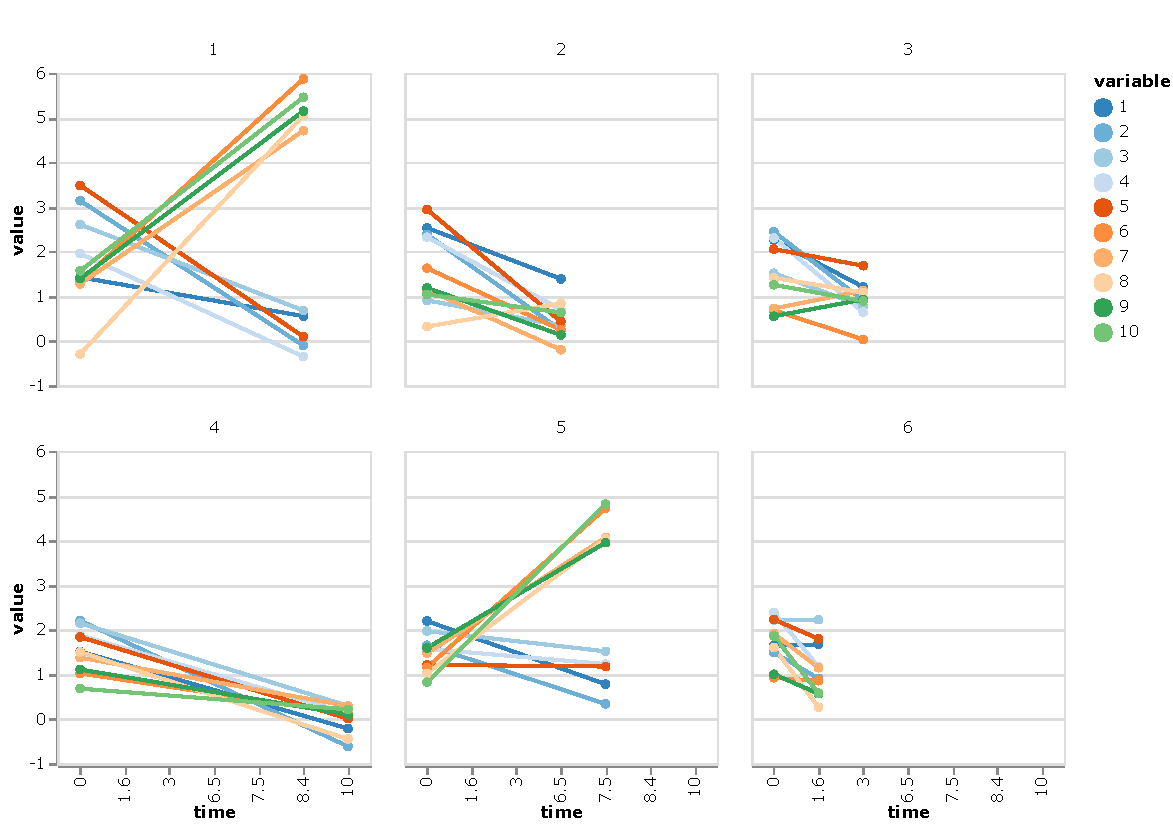
\includegraphics[width=0.8\linewidth]{exemplary_datastructure_intro.pdf}
	\caption{Exemplary data structure from simulated data. Each panel represents one individual, dots represent individual measurements and colors indicate different variables. The $x$-axis denotes the time of measurements and the $y$-axis their values.}
	\label{fig:exemplary-data}
\end{figure}

Figure \ref{fig:exemplary-data} illustrates the structure of the simulated data setting: The time point of the second measurement varies as contrasted by individuals $1$ and $6$. 
Different development patterns are reflected by two groups of individuals, one with an upward trend in some variables and a downward trend in others (e.g., individuals $1$ and $5$), and the other one with a downward trend in all the variables (e.g., individuals $2$ and $4$). 
Furthermore, the observations are characterised by groups of variables that share common trends, suggesting an underlying lower-dimensional structure. 

To build a representation of this lower-dimensional structure of the development patterns and in this way recover the central factors of variation underlying the data in an unsupervised way, I employ deep learning, specifically a variational autoencoder (VAE). I adapt the VAE and constrain its representation of the data in a latent space to model smooth trajectories by imposing an ODE system on that space. 
Furthermore, I assume inter-individual differences in development patterns to be grounded in differences in the variables measured only at baseline and use them to infer an individual-specific set of ODE parameters. 
To be able to model more complex underlying dynamics, I extend the model and enrich every individual's information by assigning to it a batch of individuals with similar underlying development patterns. The combination of all second time point measurements in the batch then serves as proxy information on the common dynamics at multiple time points. By training the model on these batches, I thus exploit the irregularity of second measurement time points to address the problem of time sparsity. 

Using the simulated data described above, I investigate the capability of the model to recover individual trajectories from both linear and non-linear two-dimensional ODE systems with two or four unknown parameters and to infer for a given observation a group of individuals with similar trajectories.

The proposed method is based on the central idea of bringing together deep learning and differential equations. This can be seen as an approach that bridges the gap between what has been referred to as the "two cultures in the use of statistical modeling to reach conclusions from data" (\cite[p.~1]{Breiman2001}): While inferring a low-dimensional latent representation in an unsupervised way directly from the data without specific assumptions on its structure with a deep neural network belongs to the "algorithmic modelling culture", the assumption of an explicit data model in the form of an underlying system of differential equations from which observations are generated with some random measurement noise represents the "data modelling culture".     

In general, formulating explicit scientific models allows to explicitly encode known structures of the data-generating forces such as physical laws or constraints into the model and treat other factors as noise, while the black-box nature of deep neural networks generally lacks interpretability. However, explicit stochastic or mechanistic data models make simplifying assumptions on the generating process that often cannot be validated. Algorithmic approaches such as neural networks have been successfully applied in many domains to approximate complex functions or learn patterns from data in an unsupervised way without explicit assumptions on the underlying data-generating process, but require large amounts of training data. 

Instead of viewing these two approaches to statistical modelling as opposing each other, recent lines of research attempt to reconcile them and combine their respective advantages: 
The methodology of universal differential equations (UDEs) developed in \cite{Rackauckas2020} aims at augmenting scientific models with machine-learnable structures as a step towards "data-efficient machine learning". With the UDEs, the authors propose differential equation models defined by a mechanistic and deterministic model that incorporates prior scientific knowledge, while a part of the equation contains an embedded black-box algorithm like a neural network that can account for missing or unobserved parts of the process. The authors employ their approach in several modelling tasks across scientific disciplines to show how UDEs can provide both interpretable and flexible models while requiring less data than pure machine learning based approaches and being efficiently trained within modern differential programming frameworks.  

My method is inspired by the recently developed neural ODEs (\cite{Chen2018}). Here, the authors introduce continuous-depth neural networks that parameterise the derivative of the hidden state and apply their idea to develop a latent continuous time-series model. While this model is also based on a VAE architecture with an ODE system governing the latent space, it assumes a fixed time grid with dense, regularly spaced observations. 
To overcome this limitation, the authors proposed an extension for irregularly sampled time series data in a follow-up work (\cite{Rubanova2019}): Originally, a recurrent neural network (RNN) with a discrete sequence of hidden states is used to encode the observed time series into a latent representation, which assumes sequences with equidistant time steps. In \cite{Rubanova2019}, this is generalised to an ODE-RNN encoder with continuously changing hidden states and an ODE specifying their dynamics. 

A conceptually similar method to model second-order ODEs within a VAE framework is presented by the ODE$^2$VAE model (\cite{Yildiz2019}). Here, the latent representation consists of a position and a velocity vector inferred separately from the input time series with an additional Bayesian network employed to handle uncertainty in the dynamics. The model does not, however, explicitly account for any uncertainty in the observation or measurement of these dynamics. 

The GRU-ODE-Bayes approach of \cite{Brouwer2019} also integrates ODE modelling with Bayesian inference, but is based on a different neural network architecture. The authors aim at continuous modelling of sporadically observed time series data with stochastic differential equations (SDEs). To this end, they combine a smooth version of the gated recurrent unit (GRU), basically a RNN with continuous instead of discrete hidden state updates similar to the ODE-RNN in \cite{Rubanova2019}, with a Bayesian update. The GRU propagates the latent state forward and allows for an update in a Bayesian fashion whenever a new observation becomes available. While the idea of alternating between a prediction and filtering step is similar to the Kalman filter, the model does not rely on the linearity or linearisation of the hidden state update and its formulation of the dynamics as ODE is better suited to model long-term dependencies and capture more complex dynamics. Since the model is not built on a VAE architecture, it neither infers a latent representation that compresses the main factors of variation in lower dimensions nor permits to generate new data samples. Although it solves a SDE and hence allows to generate trajectories by sampling paths of the SDE solution, the distribution of these trajectories is determined by the stochastic process that solves the SDE and does not necessarily account for noise factors in the original data observations.

More generally, several approaches integrate modelling of dynamic processes into a VAE architecture without using ODEs. The authors of \cite{Fortuin2019} propose a Gaussian Process-VAE (GP-VAE) that models temporal dynamics as Gaussian processes in latent space. Here, again, many time points are needed to accurately infer the Gaussian process capturing the dynamics and the time series in latent space is represented by a discrete series of steps rather than a smooth function. Consequently, the structure of the latent space does not immediately allow for inter- or extrapolation of the time series, i.e, no data can be generated for time points not observed in the training data. 

The temporal difference VAE (TD-VAE) developed in \cite{Gregor2018} is build on the idea of forming a hidden belief state that encodes a deterministic representation of the filtering posterior of the hidden state given all observations up to a specific time. This belief state is computed based on a sufficient statistic of the future given past observations and is propagated forward from one time step to the next. The model is trained by comparing observations from two (not necessarily subsequent) time points and assumes a densely and regularly sampled time grid. While the TD-VAE infers an abstract representation of the data in the hidden belief state and is able to learn from separated time points without backpropagating through the entire time interval and predict several time steps in the future, it does not learn to represent the dynamics as an explicit continuous trajectory.

Compared to the approaches mentioned above, the model proposed in this thesis is the only one inferring individual-specific dynamics by using additional baseline information and modelling individual development patterns as smooth ODE solutions based on an extremely sparse and irregular time grid of noisy measurements. The VAE architecture allows for the generation of new samples from the data distribution, while the representation of individual temporal patterns as ODE solutions permits straightforward inter- and extrapolation of the learned time series by solving the ODE at different time points than the ones originally observed.

In this thesis, I present the approach in detail. Chapter \ref{chap:background} establishes the theoretical background. In Chapter \ref{chap:methods}, I present the methodology of my approach including a derivation of the training objective and a method to realise the model extension to batches of similar individuals. 
Chapter \ref{chap:applications} is devoted to applications of the model in various simulated data settings based on different characteristics of temporal development patterns. Finally, I discuss my results, the limitations of the proposed approach and possible directions for future research in Chapter \ref{chap:discussion}. 